% Fragmento editable: solo TikZ básico, sin bibliotecas adicionales.
% Esquema prospectivo; los bloques son etapas, no módulos implementados.
% Ancho: 0.82\textwidth más dos márgenes internos de 5 pt (<16 cm).
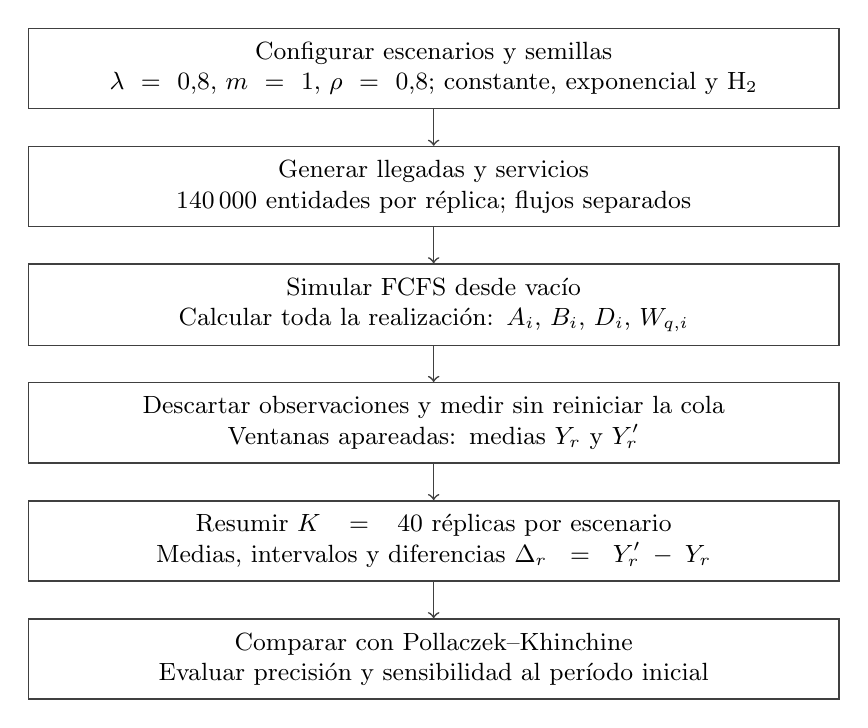
\begin{tikzpicture}[
  x=\textwidth,y=1cm,font=\small,
  etapa/.style={draw=black!75,fill=white,line width=0.5pt,
    text width=0.82\textwidth,align=center,inner sep=5pt,
    minimum height=0.95cm},
  flujo/.style={->,draw=black!75,line width=0.6pt}
]
  \node[etapa] (configuracion) at (0,0)
    {Configurar escenarios y semillas\\
     $\lambda=0{,}8$, $m=1$, $\rho=0{,}8$; constante, exponencial y H$_2$};
  \node[etapa] (generacion) at (0,-1.5)
    {Generar llegadas y servicios\\
     $140\,000$ entidades por réplica; flujos separados};
  \node[etapa] (simulacion) at (0,-3)
    {Simular FCFS desde vacío\\
     Calcular toda la realización: $A_i$, $B_i$, $D_i$, $W_{q,i}$};
  \node[etapa] (medicion) at (0,-4.5)
    {Descartar observaciones y medir sin reiniciar la cola\\
     Ventanas apareadas: medias $Y_r$ y $Y'_r$};
  \node[etapa] (resumen) at (0,-6)
    {Resumir $K=40$ réplicas por escenario\\
     Medias, intervalos y diferencias $\Delta_r=Y'_r-Y_r$};
  \node[etapa] (contraste) at (0,-7.5)
    {Comparar con Pollaczek--Khinchine\\
     Evaluar precisión y sensibilidad al período inicial};
  \draw[flujo] (configuracion.south) -- (generacion.north);
  \draw[flujo] (generacion.south) -- (simulacion.north);
  \draw[flujo] (simulacion.south) -- (medicion.north);
  \draw[flujo] (medicion.south) -- (resumen.north);
  \draw[flujo] (resumen.south) -- (contraste.north);
\end{tikzpicture}
